%In this section we show that PAT leads to better transliteration models even without parallel data.
%
%\subsection{Generative Story}


%\subsection{Parameter Agreement Training}
%In PAT, the model corresponding to the inverse generative story is also used.
%This inverse process is illustrated at the bottom of Figure \ref{fig:fsts}.
%
%The training data for the reverse direction consists of set of English pronunciations  $E=\{\mathbf{e_n}\}_{n=1}^{|E|}$ and independent training maximizes:
%\begin{align}
%L(E)& = \sum_{\mathbf{e}\in E} \log \sum_{\mathbf{j}} \QQ(\mathbf{e}\mid \mathbf{j})\cdot \QQ(j)
%\end{align}
%To apply PAT, we maximize the joint regularized objective function:
%\begin{align}
%L(J) + L(E) + \lambda R(\PP(\mathbf{j}|\mathbf{e}), \QQ(\mathbf{e}|\mathbf{j}))
%\label{eqn:dec_obj}
%\end{align}
%Once the two models are trained, Japanese words can be decoded using either model. 
%In practice we followed Ravi and Knight and used the $\PP$.
%\begin{figure*}[t]
%\begin{center}
%\begin{tabular}{ccc}
% &  & \tabularnewline
% & 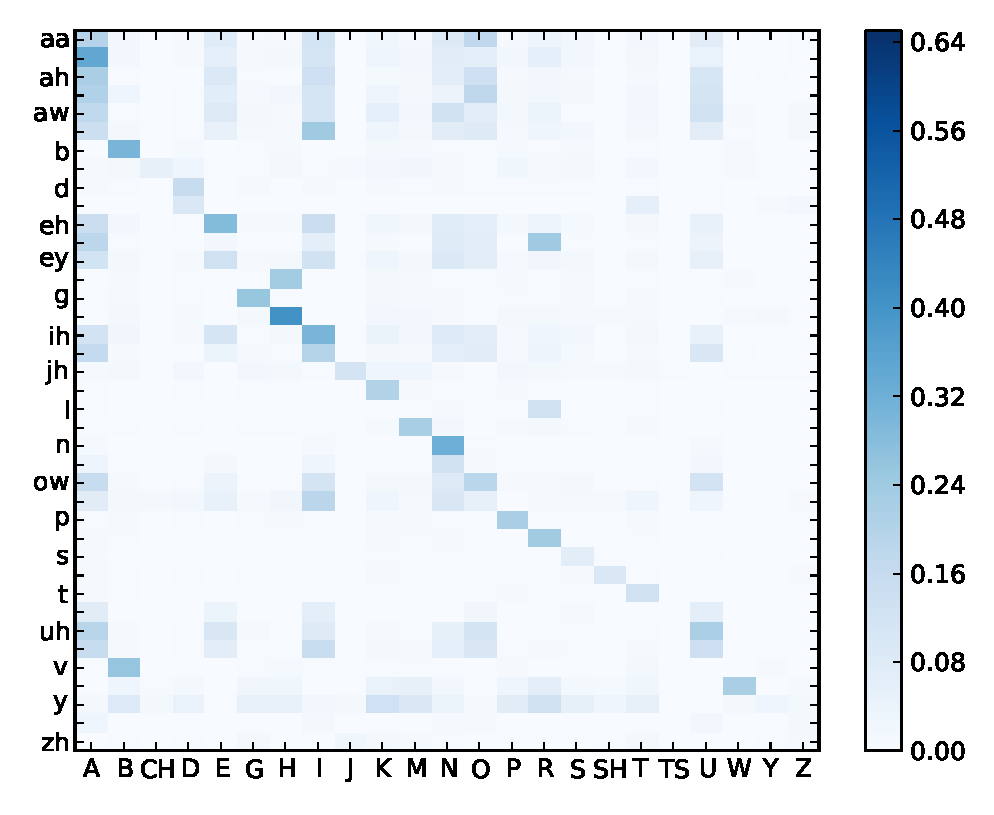
\includegraphics[scale=0.4]{figures/model_11_vanilla} &
% \includegraphics[scale=0.4]{figures/model_11_gm}\tabularnewline
% &  & \tabularnewline
%\end{tabular}
%\caption{Compared to independent training. PAT (right) learns sparser, peaked models.}
%\label{fig:mapping}
%\end{center}
%\end{figure*}

%\begin{figure*}
%\begin{center}
%\begin{tabular}{c}
%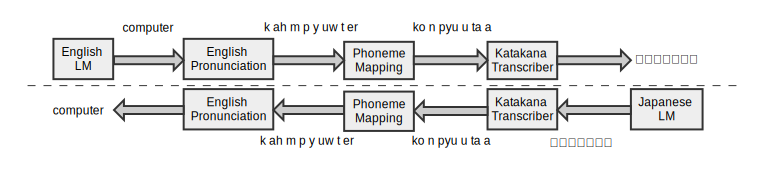
\includegraphics[scale=0.62]{figures/fsts}\tabularnewline
%\end{tabular}
%\caption{\label{font-table} The transliteration generative story as a cascade of FSTs . Each box represents a transducer. \textbf{Top:} transliteration of the word ``computer'' to Japanese. \textbf{Bottom:} the reverse process. PAT jointly trains the two cascades by maximizing both the data log-likelihood and the parameter agreement of the two (shaded) phoneme mapping models. The blank FSTs are held fixed. }
%\label{fig:fsts}
%\end{center}
%\end{figure*}

In this section we present our experiments on deciphering transliterations.
We first reproduced the English-to-Japanese transliteration pipeline of \newcite{RK09} (as described in Section \ref{sec:background} and depicted at the top of Figure \ref{fig:fsts}) and tried to match their reported results.\footnote{Unfortunately, we were unable to obtain all their FSTs and data.}
We then constructed the reverse Japanese-to-English pipeline, required for PAT, and compared the two approaches.

\subsection{The Baseline Decipherment Model}
To reproduce the English-to-Japanese pipeline, we constructed the following FST models:
\begin{enumerate}
\item A unigram language model (LM) of English terms, estimated over the top 40K most frequent capitalized words found in the Gigaword corpus (without smoothing).
\item An English pronunciation FST from the CMU pronunciation dictionary (REFERENCE?).
%http://svn.code.sf.net/p/cmusphinx/code/trunk/cmudict
\item A English-to-Japanese phoneme mapping FST that encodes the phoneme transliteration table $t_1$ (see \eqn{eqn:trans}), constructed based on the best setting reported by \newcite{RK09}. 
We note that $t_1$ is restricted to either 1-to-1 or 1-to-2 phoneme mappings, maintaining consonant parity. See further details in their paper.
\item A hand-built Japanese pronunciation to Katakana FST \cite{RK09}.
\end{enumerate}

\newcite{RK09} report back-transliteration whole-name error rates (WNER) on a list of 100 transliterated US senator names. (In WNER, a decoding is correct if both the first and last name are correctly decoded.)
They train the FST cascade in both parallel and decipherment settings, obtaining 40\% WNER in the parallel setting (trained over 3.3K word pairs) and 73\% WNER on their best decipherment setting (trained over 9.5K Japanese words only).

\subsection{The Inverse Model}
PAT requires a pipeline in the reverse direction, for transliteration of Japanese to English.
% - a Japanese-to-English transliteration pipeline with similar FST models.
We constructed a unigram LM of Katakana terms over the top 25K most frequent Katakana words found in the Japanese news 2005-2008 Leipzig corpora (REFERENCE).
%(http://corpora.informatik.uni-leipzig.de/download.html)

The remaining required FSTs were obtained by inverting the baseline FSTs (that is, FSTs 2,3,4), and the cascade was composed accordingly (depicted at the bottom of Figure \ref{fig:fsts}).
In particular, by inverting $t_1$, we obtained a Japanese-to-English FST $t_2$ that allows only 2-to-1 or 1-to-1 phoneme mappings.

\subsection{Training and Decoding}
For training data, we took the top 50\% most frequent terms from each LM, resulting in a set of 20K English terms and a set of 22.5K Japanese terms.
Using the whole set of terms led to poor baseline results, probably since uncommon English terms are not transliterated, and uncommon Katakana terms may be borrowed from languages other than English.
In any case, it is important to note that the two resulting sets of words are far from being parallel, since they were collected over non-parallel corpora.

Vanilla EM training of the baseline was done using the Carmel finite-state toolkit \cite{graehl97}.
The LM and pronunciation models were held fixed while the parameters of the phoneme mapping model $t_1$ were optimized to maximize the likelihood of the observed set of Japanese terms.

The PAT objective (\eqn{eqn:joint}) was maximized with respect to the phoneme mapping models $(\TA, \TB) = (t_1, t_2)$, with coefficient $\lambda\in\{1,2,3,4\}$.
We manipulated Carmel to compute a single E-step and output the posteriors which we then used to formulate the M-step objective. 
The M-step was solved using our own PGD implementation.\footnote{This implementation is a general purpose PGD solver for convex functions over convex closed sets, and will be released as open-source software.}

To compare against the ordinary parallel data setting, we trained the English-to-Japanese phoneme mapping model $t_1$ with Carmel. We used 4.2K pairs of English and Japanese phoneme sequences. For all models, training was limited to 15 EM iterations.

Finally, back-transliterations of Japanese terms were computed using regular Viterbi decoding of the term with the $t_1$ model only.
Note that symmetrization heuristics are not applicable, since in decipherment we have no parallel data.

\subsection{Results}
\begin{figure*}[t]
\begin{center}
\begin{tabular}{cc}
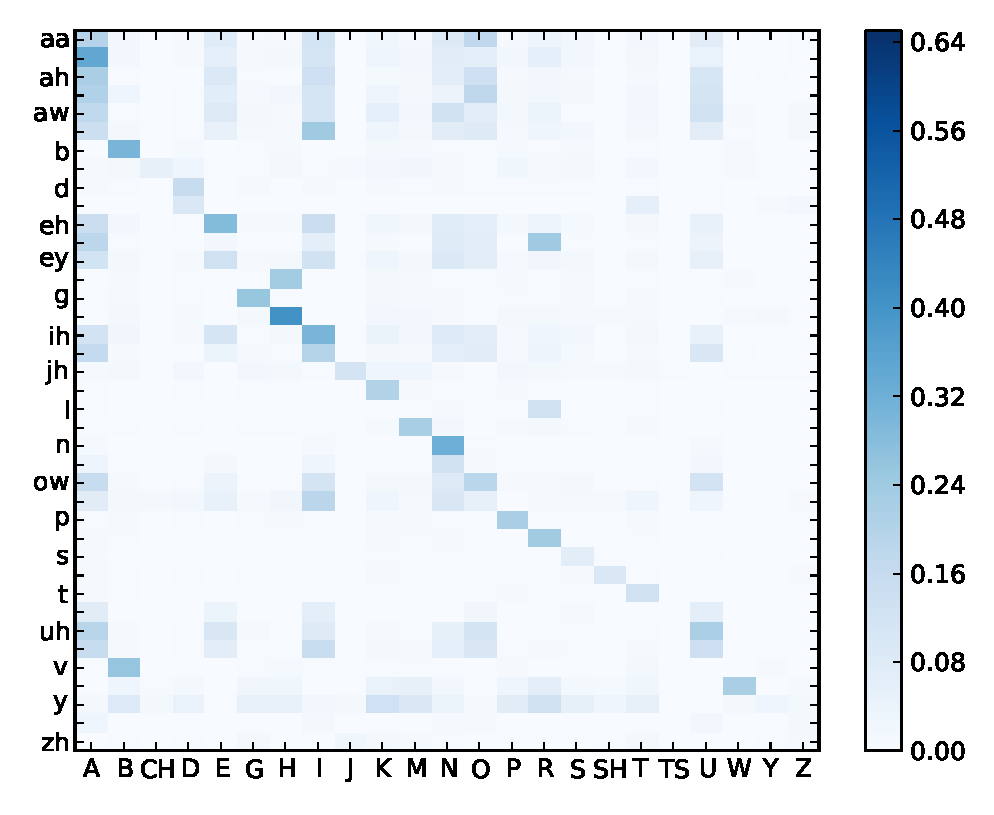
\includegraphics[scale=0.4]{figures/model_11_vanilla} & \includegraphics[scale=0.4]{figures/model_11_gm}\end{tabular}
\end{center}
\caption{The 1-to-1 mapping submatrix of the $t_1$ transliteration table. \textbf{Left}: Independent training. \textbf{Right}: our method (PAT), which learns sparser, peaked models.}
\label{fig:mapping}
\end{figure*}
We compiled our own list of 100 US senator names (first and last) to be used as a test set. 
To tune $\lambda$ we used a development set consisting of 50 frequent Japanese terms and their English origin.

For each method, we selected the $t_1$ model that minimized the development back-transliteration error rate over the 15 iterations, $\lambda$ and the so-called stretch-factor 
$\alpha \in \{1,2,3\}$ that exponentiated the model parameters before decoding (see \newcite{RK09}).

%Table \ref{tbl:transliteration}  %% ref not working for some reason
Table 1
reports WNER, average normalized edit distance (NED) and the number of $t_1$ parameters with value greater than 0.01 ($t_1>0.01$) as an indication of model sparsity. 
Figure \ref{fig:mapping} further compares a portion of the best phoneme mapping table learned by the baseline vs. that learned by PAT, depicting the difference in parameter sparsity.

\begin{table}[h]
\begin{center}
\begin{tabular}{l|c|c|c}
\multicolumn{1}{c|}{} & WNER & NED & $t_1> 0.01$\tabularnewline
\hline 
Independent & 67\% & 23.2 & 649\tabularnewline
PAT & 59\% & 17.3 & 421\tabularnewline
Parallel Data & 43\% & 10.8 & 152\tabularnewline
\end{tabular}

\caption{PAT reduces error rates (WNER, NED) and learns sparser models (number of $t_1$ parameters greater than 0.01).}
\end{center}
\end{table}

Using PAT we were able to significantly reduce the error rate, reducing the gap in WNER between independent and parallel-data settings by 33\% and the gap in NED by nearly half.
This error reduction clearly demonstrates the efficacy of jointly training these models, and of the PAT formulation in particular.



